\chapter{Compressão de Dados}
\label{chap:compressaodados}
Devido a diversos avanços tecnológicos durante as últimas décadas,
principalmente no campo de~\emph{Big Data}, a compressão de dados alcançou uma
grande importância, sendo a protagonista de muitos avanços na tecnologia atual.
Para se ter uma ideia, armazenar uma música não comprimida de apenas dois
minutos com qualidade de CD requer mais de 84 milhões de
bits~\citep{Book:IntroductionToDataCompression}, enquanto uma música no formato
MP3 de 256 kbps, também de dois minutos, requer em torno de trinta milhões de
bits, menos da metade. Em geral, a compressão pode ser definida como o
processo de conversão de uma entrada, ou o dado original, em outro dado, sendo
este a saída, ou o dado comprimido, cujo tamanho é inferior à entrada. Na
Computação, o conceito de tamanho é aplicável à quantidade de bits que se
utiliza para a representação de um dado.

Embora a compressão esteja sendo amplamente explorada nos dias de hoje, esta é
uma área de estudos precedente à própria Computação. Alguns autores atribuem a Samuel
Morse o primeiro projeto de compressão de dados. Samuel criou, em 1835,
o Código Morse, sistema pelo qual era possível enviar mensagens a partir de um telégrafo,
onde os caracteres de um texto eram trocados por sequências de pontos e traços.
Samuel percebeu que o aparecimento de algumas letras era mais comum que outras
em um texto, e atribuiu a elas uma sequência de pontos e traços mais curtas que
caracteres que menos apareciam. Por exemplo, a letra \emph{E} é representada por
apenas um ponto ($\bullet$) enquanto a letra \emph{X} é representada pela
sequência traço, ponto, ponto, traço (--- $\bullet~\bullet$ ---).

Nos anos que se seguiram à invenção de Samuel, avanços substanciais foram feitos
no campo da Teoria da Informação, com especial atenção ao artigo de Claude
Elwood Shannon~\citep{Artigo:EntropiaShannon}. Shannon descreve, entre outros
conceitos, o de~\emph{entropia} como medida de informação. A entropia estabelece
a menor média de bits necessária para se representar um dado sem perdas. Seu
conceito foi baseado na divisão do dado em símbolos com suas respectivas
probabilidades. Dessa forma, um~\emph{símbolo} é a menor parte em que um dado é
subdividido. Por exemplo, em um texto o conjunto de símbolos únicos pode ser
cada caractere isolado (letra, espaço, pontuação etc.) dele. É possível escolher
também cada palavra do texto como elemento do conjunto de símbolos. A entropia está
representada matematicamente na Equação~\ref{eq:entropia}, onde $n$ é o número
de símbolos distintos do dado e $P_i$ é a probabilidade de cada símbolo ocorrer.

\begin{equation}
\displaystyle H = - \sum_{i=1}^{n}P_i\log_2P_i
\label{eq:entropia}
\end{equation}

Para calcular a entropia da frase~\emph{O rato roeu a roupa do rei de Roma}, por
exemplo, considerando que cada letra seja um símbolo, que todas as letras são
minúsculas e sem considerar o caractere espaço, é necessário, primeiramente,
calcular a probabilidade de cada símbolo único aparecer e, depois, $\log_2P_i$.
Tais cálculos podem ser vistos na Tabela~\ref{Tabela:Oratoroeu}. Em seguida,
aplicando a Equação~\ref{eq:entropia} nos dados da Tabela~\ref{Tabela:Oratoroeu}
obtem-se o valor $H = 3,013$ bits por símbolo. Em outras palavras, cada símbolo
ocuparia, em média, $3,013$ bits. Como a mensagem possui $26$ símbolos, o
tamanho total a ser ocupado é de $26 \times 3,013 \approx 79$ bits. Na
codificação UTF-8, cada símbolo ocupa 8 bits, $8 \times 26 = 208$ bits. Bem
acima da entropia calculada.

\begin{table}[ht]
\centering
\begin{tabu}{c|c|c|c}
\tabucline[2pt]{-}
\textbf{Caractere} & \textbf{Nº aparições} & $P_i$ & $\log_2P_i$ \\ \tabucline[2pt]{-}
t, p, m, i & 1 & 0,038462 & -4,70044
 \\ 
\hline 
%p & 1 & 0,038462 & -4,70044 \\ 
%\hline 
%m & 1 & 0,038462 & -4,70044 \\ 
%\hline 
%i & 1 & 0,038462 & -4,70044 \\ 
%\hline 
d, u & 2 & 0,076923 & -3,70044 \\ 
\hline 
%u & 2 & 0,076923 & -3,70044 \\ 
%\hline 
e & 3 & 0,115385 & -3,11548 \\ 
\hline 
a & 4 & 0,153846 & -2,70044 \\ 
\hline 
r & 5 & 0,192308 & -2,37851 \\ 
\hline 
o & 6 & 0,230769 & -2,11548 \\ 
\tabucline[2pt]{-}
\end{tabu} 
\caption[Probabilidade e $\log_2$ dos símbolos distintos do
exemplo]{Probabilidade e $\log_2$ dos símbolos distintos da frase
\emph{O rato roeu a roupa do rei de Roma}.}
\label{Tabela:Oratoroeu}
\end{table}

Uma crítica a ser feita ao conceito de entropia estabelecido por Shannon é que
ele não leva em consideração a autocorrelação do dado. Portanto, é possível
reduzir a entropia de um dado removendo sua redundância. Os
termos~\emph{redundância},~\emph{estrutura},~\emph{padrão}
e~\emph{autocorrelação} referem-se a um mesmo conceito na área de
compressão~\citep{Book:DataCompressionTheCompleteReference}. Em geral, um dado
qualquer de natureza não puramente aleatória possui uma coleção de padrões, que pode
ser explorada a fim de se obter uma representação da informação original
utilizando um número menor de bits. 

Levando-se em conta que em geral a informação é correlacionada, muitos autores
lançam mão de uma abordagem em duas etapas, sendo a primeira a decorrelação do
dado \label{Paragrafo:descorrelacaoprimeiraetapa} e redução de sua variância e a
segunda a utilização de um algoritmo de compressão em si. Esse paradigma não é
novidade e já foi abordado em outros
trabalhos~\citep{Article:twostagecompression}.
A Figura~\ref{Figura:compressaoduasetapas} ilustra o processo de compressão em
duas etapas. %Na teoria, qualquer método capaz de produzir resultados com as
% caracteríticas supracitadas pode ser usado na primeira fase de compressão. Por
% agora, a discussão dos métodos existentes na prática será suspensa e somente
% retomada no capítulo~\ref{Capitulo:propostatrabalho}, quando alguns trabalhos
% relacionados forem descritos.

\begin{figure}[htb]
\centering
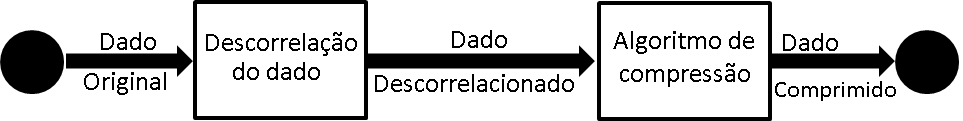
\includegraphics[scale=0.5]{fig/twostagecomp.png}
\caption[Compressão de duas etapas]{Esquema de compressão em duas etapas. Na
primeira, o dado é descorrelacionado para que sua entropia seja diminuida. Na
segunda, um algoritmo de compressão é utilizado.}
\label{Figura:compressaoduasetapas}
\end{figure}

Na segunda etapa, algoritmos clássicos de compressão são utilizados. Como a
solução criada em 1952 por David Albert Huffman e publicada 
em~\citep{Artigo:CodigoHuffman}. A Codificação de Huffman. Uma ideia tão simples
que, segundo~\citep{Book:HuffmanWinZip2}, \textquotedblleft até um aluno do
Ensino Médio poderia entender\textquotedblright. A ideia de Huffman se valia da
probabilidade de cada símbolo único ocorrer no dado de entrada. O algoritmo
baseia-se na criação de uma árvore binária onde cada nó representa um símbolo
do dado. Símbolos com maior número de repetições no dado original
estão mais perto da raiz, enquanto que aqueles com menor probabilidade possuem
maior altura na árvore. Atribuindo-se o bit um aos filhos à esquerda e zero aos
da direita de um nó, obtem-se a nova codificação do símbolo percorrendo a
árvore. 

A Codificação de Huffman é um algoritmo guloso~\citep{Livro:cormen} e é
tida hoje como o primeiro método moderno de compressão existente~\citep{Book:LosslessCompressionHandbook} e utilizado em
programas como Winzip e PKZip~\citep{Book:HuffmanWinZip, Book:HuffmanWinZip2}.
Nos anos que se seguiram, foram feitas diversas tentativas de tornar a
Codificação de Huffman dinâmica, ou seja, capaz de calcular a probabilidade de
cada símbolo aparecer em tempo real, ajustando a árvore construída
dinamicamente sempre que necessário. Destacam-se as soluções propostas
em~\citep{Artigo:KnuthDynamicHuffman} e~\citep{Artigo:VitterDynamicHuffman}.

%Na década de 1960, a Codificação Aritmética, um dos algoritmos mais
%usados nos dias de hoje, utilizado em dezenas, talvez
%centenas de patentes, foi descrita em~\citep{Book:ArithmeticCoding}. A
%Codificação Aritmética também será utilizada nesse trabalho e, por esta razão,
%será explicada mais detalhadamente na seção~\ref{Subsec:CodificacaoAritmetica}.

Outra solução que pode ser usada na segunda etapa é a Codificação
Aritmética~\citep{Book:ArithmeticCoding}.
Como ela será utilizada nesse trabalho, ela será detalhada na
seção~\ref{Subsec:CodificacaoAritmetica}.

\section{A Codificação Aritmética}
\label{Subsec:CodificacaoAritmetica}

A Codificação Aritmética, proposta primeiramente
em~\citep{Book:ArithmeticCoding} e estudada mais a fundo
por~\citep{Artigo:ArithmeticCoding}, faz parte de um dos algoritmos de
compressão mais utilizados atualmente, seja diretamente ou como base para
outras soluções. Diferente dos demais algoritmos, como o de Huffman,
a codificação aritmética não cria um código único para cada símbolo distinto do
dado e depois relê o dado original substituindo cada símbolo pelo seu respectivo
código, ela gera um código que representa todo o dado de
entrada, de forma que trocar dois símbolos de lugar pode criar um código
completamente diferente do anterior. Já na codificação de Huffman, por exemplo,
o código só mudaria nas posições onde houve a troca.

O objetivo do algoritmo é gerar um número entre zero e um a partir do qual o
dado original seja regerado. Como entrada, o algoritmo precisa da probabilidade
de aparecimento de cada símbolo único existente no dado original. O seu
primeiro passo consiste em criar o intervalo $(0, 1]$ e particioná-lo na mesma
quantidade de símbolos distintos do dado original. Cada partição representa um
dos símbolos distintos do dado original, é rotulada de acordo com o símbolo que
representa e possui tamanho proporcional à probabilidade do respectivo símbolo.

No próximo passo, o algoritmo lê o primeiro
símbolo do dado de entrada, encontra a partição a que pertence tal
símbolo e redimensiona o intervalo, que antes era $(0, 1]$, para o tamanho
referente à partição do símbolo lido. Esse processo é repetido para cada
um dos próximos símbolos existentes no dado de entrada, até que eles terminem.

Existe uma técnica capaz de escolher o
melhor número no intervalo calculado na codificação aritmética e facilitar a
decodificação do dado comprimido. Ela se baseia em uma busca binária no
intervalo original, que inicialmente era $(0, 1]$. Nessa condição, o primeiro
número testado seria $0,5$. Se $0,5$ estiver contido no intervalo calculado pela
codificação aritmética, $0,5$ é transformado em binário e enviado ao
decodificador. Se não, testa-se se $0,5$. Se ele for menor do que o limite
inferior do intervalo calculado pela codificação aritmética, o próximo número a ser testado
é $0,75$. Se $0,5$ for maior que o limite superior do intervalo, o próximo
valor a ser testado é $0,25$. Esse processo se repete até que o primeiro número
dentro do intervalo calculado pela codificação aritmética seja encontrado. Este
número é transformado em binário e enviado ao decodificador. %e retornado pela
% função. % O algoritmo~\ref{alg:codifarit} ilustra esse processo.

%O objetivo do~\emph{Arithmetic Encoding} é codificar o dado de entrada gerando
%um número entre zero e um a partir do qual a sequência original possa ser
%recuperada, sem perdas. Diferente de outros métodos de compressão por redução
% de entropia, como o algoritmo de Huffman, que calculam uma sequência distinta
% de bits para cada símbolo, o Arithmetic
%Coding gera uma sequência a partir de todo o dado de entrada.

%Para a compressão, o \emph{Arithmetic Encoding} necessita do dado original e da
%probabilidade de cada símbolo ocorrer para codificar o dado. No início, o
%algoritmo trabalha com um intervalo largo $[0, 1)$ e o vai diminuindo conforme
%novos dados do conjunto a ser codificado são lidos. Símbolos com maior
%probabilidade de aparecimento diminuem o intervalo mais suavemente, enquanto
%os com menor probabilidade achatam o intervalo com mais veemência. O algoritmo
%está abaixo.

%\begin{algorithm}[ht]
%\caption{A Codificação Aritmética}
%\label{alg:codifarit}
%\Entrada {\\ \textbf{\emph{dadoOriginal}} - O dado que se deseja comprimir. \\
%\textbf{\emph{probSimbolos}} - Tabela de dispersão onde uma chave representa um
%símbolo único do dado e o valor dessa chave a probabilidade de tal símbolo
%aparecer.}
%\vspace{1mm}
%\Saida{\\ \textbf{\emph{codificado}} - um número binário a partir do qual o
%dadoOriginal pode ser reconstruído.}
%\vspace{1mm}
%\hrule
%\vspace{1mm}
%\SetKwFunction{rec}{$\leftarrow$}
%\Inicio
%{
%    tamIntervalos \rec probSimbolos.clone()\; 
%    \ParaCada{simboloAtual $\in$ dadoOriginal}
%    {
%    	probAtual \rec probSimbolos [simboloAtual]\;    	%
%		tamIntervalos \rec tamIntervalos $\times$ probAtual\
%    }
%    
%    limite\_inferior \rec min(tamIntervalos.values())\; 
%    limite\_superior \rec max(tamIntervalos.values())\;
%    numero \rec encontra\_melhor\_numero(limite\_inferior, limite\_superior)\; 
%    resposta \rec passa\_para\_binario(numero)\;
%    \Retorna resposta\;
%}
%\end{algorithm}

%A probabilidade de cada símbolo único será exaustivamente consultada no
% decorrer do algoritmo. Por esta razão, optou-se por utilizar uma tabela de dispersão,
%onde os símbolos únicos do dado original são utilizados como chave, e a
%probabilidade do respectivo símbolo o valor associado a ela.

Seja o dado original $A = \{a_1, a_1, a_2, a_1, a_1\}$ e o conjunto de
probabilidades $P = \{P_{a_1} = 0,8; P_{a_2} = 0,2\}$. Deseja-se utilizar a
codificação aritmética para comprimir $A$. Primeiramente, o intervalo $[0, 1)$
é particionado em duas partes, já que existem apenas dois símbolos distintos no
dado original, $a_1$ e $a_2$. Como a probabilidade de $P_{a_1} = 0,8$ e
$P_{a_2} = 0,2$, esse é o tamanho das partições de $a_1$ e $a_2$,
respectivamente. Em seguida, os dados começam a ser lidos. $a_1$ é o primeiro
elemento de A. Como a partição de $a_1$ no intervalo original é delimitada por
$[0,2; 1)$, esses serão os novos limites do intervalo.

A Figura~\ref{fig:arithmeticencoding} ilustra esse processo por iteração. Na
primeira iteração, o intervalo original $(0, 1]$ é calculado, este intervalo é
cortado em $0,2$, formando duas novas partições. Exatamente o mesmo número de
símbolos distintos existentes no dado de entrada. O intervalo é particionado em
$0,2$ justamente porque esta é a probabilidade do símbolo $a_2$ aparecer. O
algoritmo lê o primeiro dado do símbolo original ($a_1$), encontra a partição a
que ele pertence e redimensiona o intervalo para $(0,2, 1]$. Na iteração dois, o
segundo símbolo do dado original é lido ($a_1$) e o intervalo, que antes estava
limitado por $(0,2, 1]$ agora é redimensionado e limitado por $(0,36, 1]$. Na
terceira iteração, o terceiro símbolo do dado original é lido ($a_2$). Agora, a
partição rotulada de $a_1$ é escolhida, e o intervalo original do algoritmo
passa a ser $(0,36, 0,488]$, tamanho da partição de $a_1$ na iteração três. Esse
processo continua até que não existam mais dados a serem lidos.

Uma vez que os símbolos no dado original terminam, tem-se um último intervalo,
delimitado pelo menor e maior tamanhos de partições, respectivamente. Qualquer
número contido nesse intervalo pode ser enviado para o decodificador para que,
junto com as probabilidades de cada símbolo ocorrer, o dado original seja
regenerado, sem perdas.

\begin{figure}[ht]
\centering
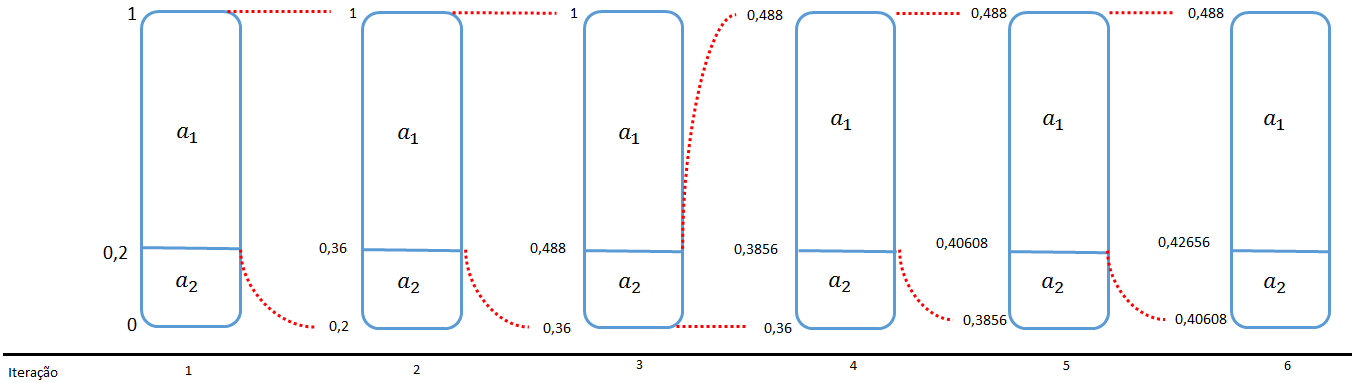
\includegraphics[scale=0.45]{fig/arithmeticencoding.png}
\caption[Ilustração do algoritmo da codificação aritmética]{Ilustração do
algoritmo da codificação aritmética}
\label{fig:arithmeticencoding}
\end{figure}


De acordo com a Figura~\ref{fig:arithmeticencoding}, qualquer número no
intervalo $[0,40608; 0,488)$ pode ser enviado para o decodificador para que haja
a descompressão. Para se escolher o melhor número no intervalo, faz-se uma busca
binária como acima mencionado. O primeiro número testado é $0,5$, pois $(1 + 0)
/ 2 = 0,5$. Como $0,5$ está acima do intervalo superior $0,488$, o próximo valor a
ser testado é $0,25$, pois $(0 + 0,5) / 2 = 0,25$, que está abaixo do intervalo
inferior $0,40608$. A Tabela~\ref{Tabela:codificacaoaritmeticaexemplo} mostra as
iterações do algoritmo de busca binária à procura do primeiro número dentro do
intervalo calculado pela codificação aritmética. O número encontrado foi
$0,4375$.

\begin{table}[ht]
\centering
\begin{tabu}{c|c|c|c}
\tabucline[2pt]{-}
\textbf{Intervalo Inferior} & \textbf{Intervalo Superior} & \textbf{Valor
Testado} & \textbf{Situação} \\
\tabucline[2pt]{-} 0 & 1 & 0,5 & < superior
 \\ 
\hline  
0 & 0,5 & 0,25 & < inferior \\ 
\hline 
0,25 & 0,5 & 0,375 & < inferior \\ 
\hline 
0,375 & 0,5 & 0,4375 & Dentro do intervalo \\ 
\tabucline[2pt]{-}
\end{tabu} 
\caption[Iteração algoritmo codificação aritmética]{Exemplo iteração algoritmo
codificação aritmética}
\label{Tabela:codificacaoaritmeticaexemplo}
\end{table}

Para a descompressão, o valor $0,4375$ bem como a probabilidade de cada símbolo
único ocorrer são suficientes. Algumas implementações também pedem a quantidade
de símbolos existentes no dado original para facilitar o processo. A grande
vantagem da codificação aritmética é que ela tende para a entropia do dado. Em
outras palavras, seja um dado hipotético de tamanho infinito, é possível provar
que a entropia do dado gerado pela codificação aritmética tende a $H$
(equação~\ref{eq:entropia})~\citep{Artigo:ArithmeticCoding}. Como desvantagens,
a codificação aritmética sofre do risco de truncamento, caso o número calculado
pelo algoritmo contenha muitas casas decimais. Ademais, a codificação aritmética
foi projetada para funcionar com números inteiros e em intervalos contínuos.
 
 %Em linhas gerais, o algoritmo inicia com um intervalo entre zero e um,
 %particiona-o em $k$ pedaços, sendo $k$ o número de símbolos únicos no dado
 %original. Cada pedaço tem o tamanho proporcional à probabilidade do símbolo
 %aparecer e receberá um rótulo para identificar o símbolo a que ele pertence.
 
 %A partir de então, o algoritmo lê cada símbolo do dado original, encontra a
 %partição referente àquele símbolo e assume o intervalo atual como o da
 %% partição do símbolo encontrado. Dessa forma, o intervalo que antes variava
 % entre $[0,
 %1)$, agora varia de acordo com o intervalo $[SP_{s - 1}, SP_{s - 1} +
 % SP_{s})$, onde $SP_{s-1}$ representa a soma dos tamanhos das partições
 % anteriores à do
 %símbolo atual e $SP_s$ o tamanho da partição atual. Essa operação é repetida
 % enquanto houver símbolos no dado original a serem lidos.
		
%A grande vantagem do \emph{Arithmetic Encoding} é que ele chega perto da
% entropia do dado, sem que haja um pré-requisito nele (por exemplo, a
% codificação de Huffman só alcança a entropia máxima se a probabilidade dos
% símbolos ocorrerem forem potências de dois). A desvantagem do  \emph{Arithmetic
% Encoding} é que, quanto mais símbolos distintos o dado original possui, mais
% ineficiente a compressão se torna, pois símbolos que pouco aparecem diminuem o
% intervalo bruscamente, aumentando a quantidade de casas decimais a serem
%enviadas para o decodificador. 

%O \emph{Arithmetic Encoding} é adequado quando se percebe que o número de
%ocorrências de um símbolo no dado é muito maior que a soma das ocorrências dos
%demais. Uma vantagem do algoritmo é que, nessas condições, ele chega
%perto da entropia do dado. Uma desvantagem é que o algoritmo não funciona bem
%com um número grande de símbolos.

%\subsection{O algoritmo de Stearns}

%Para contornar os problemas descritos anteriormente, Stearns propôs
%em~\citep{Artigo:stearn} um método para limitar a quantidade de símbolos do
%dado original. A ideia é fazer com que o Arithmetic Coding visualize vários
% símbolos como um só. Para isso, criam-se os vetores chamados~\emph{bin}
% e~\emph{offset}.
%Além disso, mais um parâmetro é escolhido, o~\emph{nbin}, que significa quantos
%símbolos o Arithmetic Coding deve enxergar.

\subsection{O algoritmo de Stearns}
\label{Paragrafo:stearns}

Para contornar os problemas acima citados, Stearns
propôs um método para limitar a quantidade de símbolos do dado original e
transformá-los em inteiros~\citep{Artigo:stearn}. O algoritmo de Stearns deve
ser rodado antes do dado ser enviado à codificação aritmética. Seja $A$ o dado
que se deseja comprimir utilizando codificação aritmética, Stearns propõe que
todos os elementos de $A$ sejam divididos por um mesmo valor. Essa divisão deve
ser inteira. Posteriormente, o resto das divisões por esse mesmo valor 
deve ser calculado. Dessa forma, de $A$ foram obtidas duas novas séries
numéricas $A_B$, com os quocientes das divisões e $A_O$ com os restos. Ambas
inteiras.
 
Idealmente, espera-se utilizar um divisor que crie muitos valores repetidos em
$A_B$, de forma que a contagem de elementos em $A_B$ siga uma distribuição
gaussiana. A contagem de elementos de $A_O$, em contrapartida, deve gerar uma
distribuição uniforme. $A_B$ é, então, comprimido com codificação aritmética e
$A_O$ não sofre qualquer compressão. 

O Algoritmo~\ref{Algoritmo:Stearns} descreve a criação de Stearns. As linhas 2
e 3 nada mais fazem do que iniciar os vetores $A_O$ e $A_B$. A
função~\emph{zeros} retorna um vetor de $|A|$ elementos, todos iguais a zero.
Na linha 4, o contador $i$ é iniciado. A linha 5 estabelece a condição de parada do algoritmo,
já que $|A|$ designa o número de elementos de A.

A linha 6 indica que o resto da divisão do elemento na posição $i$ do vetor A
por nbin será guardado na posição $i$ do vetor $A_O$. Na linha 7, o quociente,
arredondado para baixo, da divisão do elemento na posição $i$ do vetor A por
nbin é guardado na posição $i$ do vetor $A_B$. A linha 8 incrementa o índice
atual dos vetores e a linha 10 retorna o resultado obtido.

\begin{algorithm}[ht]
\caption{Algoritmo desenvolvido no trabalho de~\citep{Artigo:stearn} para
diminuir o número de símbolos para compressão com a codificação aritmética}
\label{Algoritmo:Stearns}
\Entrada 
{
\begin{description}
  \item[A]\\
  	Vetor contendo o conjunto de números sobre os quais deseja-se aplicar o
  	algoritmo de Stearns
  \item[nbin]\\
  	Número inteiro indicando o número máximo de símbolos distintos que \textbf{A}
  	deve conter
\end{description}
}
\vspace{1mm}
\Saida
{
\begin{description}
  \item[$A_O$]\\
  	Vetor de restos das divisões.
  \item[$A_B$]\\
  	Vetor com o quociente das divisões.
\end{description}
}
\vspace{1mm}
\hrule
\vspace{1mm}
\SetKwFunction{rec}{$\leftarrow$}
\Inicio
{
	$A_O$ \rec zeros($|A|$)\;
	$A_B$ \rec zeros($|A|$)\;
	i \rec 0\;
	\Enqto{i $< |A|$ }
	{
		$A_O$[i] \rec resto\_divisao(A[i], nbin)\;
		$A_B$[i] \rec $\displaystyle \floor[\Bigg]{\frac{A[i]}{nbin}}$\;
		i++\;
	}
	\Retorna $\{A_O, A_B\}$\;
}
\end{algorithm}

Suponha o vetor $A = \{52, 54, 55, 50, 53, 58, 47, 51, 56, 59\}$ e o valor de
nbin igual a 10. A aplicação do algoritmo de Stearns resultaria nos vetores
$A_B = \{5, 5, 5, 5, 5, 5, 4, 5, 5, 5\}$ e $A_O = \{2, 4, 5, 0, 3, 8, 7, 1, 6,
9\}$. $A_B$ é então comprimido pela codificação aritmética e $A_O$ é enviado
para o decodificador sem nenhum tipo de compressão.

\begin{figure}[ht]
\centering
\begin{subfigure}{.49\textwidth}
  \centering
  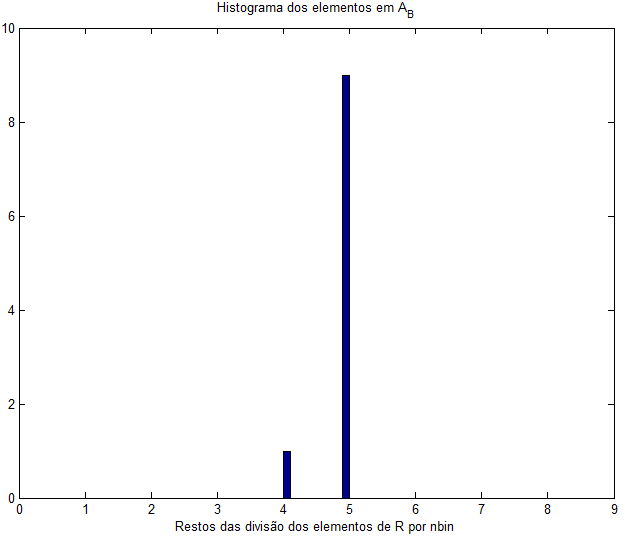
\includegraphics[width=1\linewidth]{fig/histxb.png}  
  \caption{Histograma dos quocientes das divisões dos elementos de A por nbin.}
  \label{fig:histab}
\end{subfigure}%
\hfill
\begin{subfigure}{.49\textwidth}
  \centering
  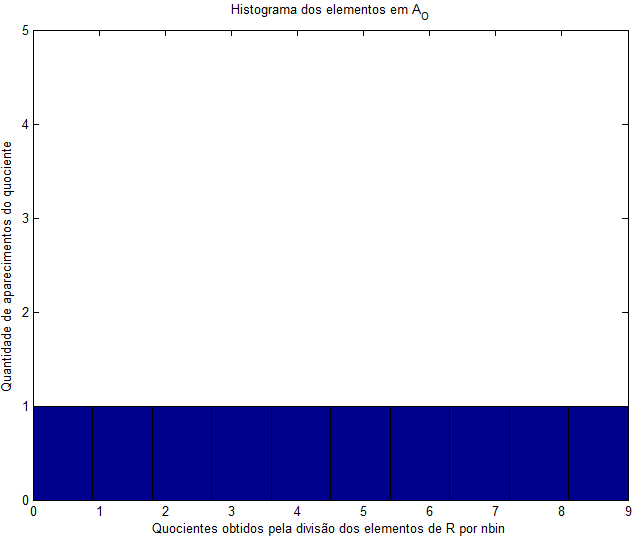
\includegraphics[width=1\linewidth]{fig/histxo.png}
  \caption{Histograma dos restos das divisões dos elementos de A por nbin.}
  \label{fig:histao}
\end{subfigure}
\caption[Histogramas gerados pela aplicação do algoritmo de Stearns]{À esquerda
o histograma segue uma distribuição gaussiana.
À direita o histograma segue uma uma distribuição uniforme. Esse é o resultado ideal da
aplicação do algoritmo de Stearns.}
\label{fig:naoestacionariaeestacionaria}
\end{figure}
